\documentclass[10pt,a4paper]{article}
\usepackage{graphicx}
\usepackage{datetime}
\usepackage{color}
\usepackage[ latin1 ]{ inputenc }
\usepackage{wrapfig}
\usepackage{ mathpazo }
\usepackage[ T1 ]{ fontenc }
\usepackage[font+=small]{sub caption}
\usepackage[font=small,labelfont=bf]{caption}
% load some useful math symbols / fonts
%\usepackage{ latexsym , amsfonts , amsmath , amssymb }
\usepackage[top =1 in ,bottom =1in ,left =1 in ,right =1 in ]{geometry}
\usepackage{natbib}
% control some spacings
%
% spacing after a paragraph
\setlength{\parskip }{.15 cm }
% indentation at the top of a new paragraph
\setlength{\parindent }{0.0 cm }
\begin{document}
\begin{figure}[h!]
	\begin{subfigure}[b]{0.51\textwidth}
		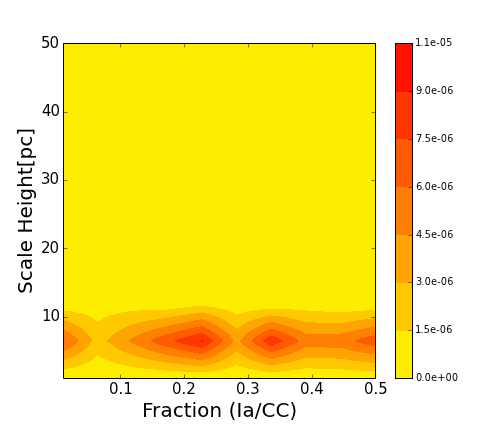
\includegraphics[width=9cm]{7.png}
		\caption{}
	\end{subfigure}
	\begin{subfigure}[b]{0.5\textwidth}
		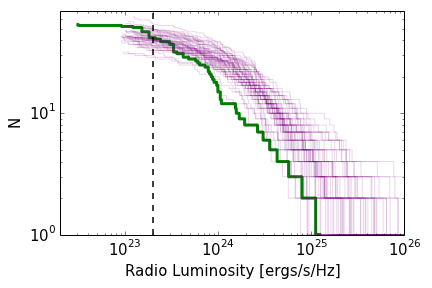
\includegraphics[width=8cm]{LumHist_f01d1.png}
		\caption{scale height=1pc, fraction = 0.1}
	\end{subfigure}
	\begin{subfigure}[b]{0.5\textwidth}
		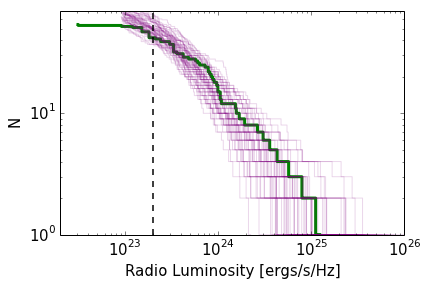
\includegraphics[width=8cm]{LumHist_f022d6.png}
		\caption{scale height = 6 pc, fraction = 0.22}
	\end{subfigure}
	\begin{subfigure}[b]{0.5\textwidth}
		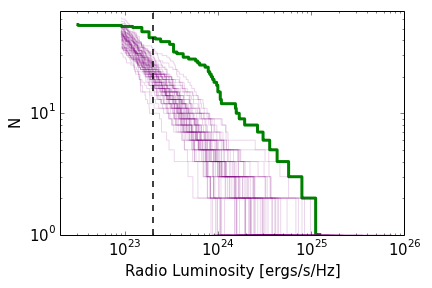
\includegraphics[width=8cm]{LumHist_f30d04.png}
		\caption{scale height = 30 pc, fraction = 0.4}
	\end{subfigure}
	\caption{Fig 1a. shows the scale height-fraction of Ia/CC parameter space. The color-bar shows the likelihood values. Fig. 1[b-c] shows the cumulative histograms of the observed (green) luminosities compared to the model luminosities (purple) for 50 snapshots, for given values of fraction and scale height. The vertical dashed line is the luminosity cutoff, above which i'm doing my model-observation comparison.\\\\ \textbf{NOTE}: Don't trust the contours in Fig 1a. since I used interpolation to construct them from (10x10) data points. Nevertheless, you can still see the "good" areas of the parameter space.}
\end{figure}
\noindent\makebox[\linewidth]{\rule{\paperwidth}{0.4pt}}
\textbf{METHOD} : I divided the observed luminosities into 5 bins, calculated the Poisson probabilities of getting the observed number of remnants per bin, given the expectation from the model (given value of scale height and fraction, averaged over 50 snapshots), and then the likelihood by multiplying the probabilities. All this is in accordance with the method in Badenes[2010] paper.\\\\
\textbf{RESULTS}
I plot the parameter space of scale height-fraction from the likelihoods in Fig 1a. This is a much more robust and consistent method than the KS-Test that I did earlier, as you can infer from the visuals in Fig. 1[b-d]. We can clearly rule out areas of parameter space. Unfortunately, the best-fit values of thickness(5-10 pc) is much lower compared to the literature (80 pc for HI in the Milky Way, Ferriere [2001], 100 pc in Magellanic Clouds, Badenes [2010]). I have two things in mind that \emph{could} fix this :-
\begin{itemize}
	\item Revisiting the light curve model. 
	\item Incorporating varying kinetic energy of SNRs in the model.
	\item Modifying the vertical density distribution (gaussian) profile of the galaxy.
\end{itemize}

 
\end{document}